% Main file of the paper. Build: latexmk -pdf main.tex   (from paper/)
% Each section lives in sections/<name>.tex.
\documentclass[11pt,a4paper]{article}

\usepackage[utf8]{inputenc}
\usepackage[T1]{fontenc}
\usepackage{lmodern}
\usepackage[margin=2.5cm]{geometry}
\usepackage{amsmath}
\usepackage{graphicx}
\usepackage{booktabs}
\usepackage[numbers,sort&compress]{natbib}
\usepackage[hidelinks]{hyperref}

\graphicspath{{figures/}}

\title{In-Situ Re-optimization of Gravitational-wave Detector Coatings\\
       for Improved Deposition Error Tolerance}
\author{Tasdik Ahmed Tonmay\\
        \small Notre Dame College, Dhaka, Bangladesh}
\date{}

\begin{document}
\maketitle

\begin{abstract}
Optical coatings used in gravitational-wave detectors such as Advanced LIGO consist of multiple thin layers (${\sim}40$). Their thicknesses must be precisely controlled to meet stringent optical specifications. However, deposition errors can still occur due to imperfect deposition tools, which, in turn, can cause finished mirrors to deviate from their target specifications. In this paper, we investigate whether these deviations can be corrected during manufacturing by measuring the deposited layers and re-optimizing the thicknesses of the remaining layers. We call this procedure rescue. For this project, we used computer simulations of a 40-layer Advanced LIGO-style mirror coating. We simulated 32 different mirror coating designs that satisfy the required transmission targets at 1064~nm and 532~nm. Our simulations show that the success of rescue highly depends on the precision of measurements. For example, for independent, layer-to-layer deposition errors and perfect measurements, the rescue of the top 4 layers raised the largest error that still lets 95\% of mirrors pass from 1.14\% to 1.71\% for the typical (median) design. This method improved the tolerable error in 30 out of 32 designs, and re-optimizing 6 to 8 layers gave higher pass rates still. With 1\% measurement error, we still got improvement in 25 out of 32 designs. However, when measurement error reached 2\%, it reduced performance in 25 designs. Rescuing only the mirrors predicted to fail reduced this harm but did not remove it. Across all the cases we tested, the rescue helped only when the measurement error was smaller than the deposition error. Under fully shared deposition errors, the rescue produced only modest improvements: the median pass rate at 1\% error increased from 66\% to 76\%, but no design achieved a 95\% pass rate. Even with 12 re-optimized layers, only 2 of the 32 designs reached it, and a global optimizer did not help. The full thermal-noise calculation showed a negligible change: the median changed by $-0.02\%$.

These results suggest that in-process re-optimization can improve coating tolerance to independent deposition errors, provided that layers are measured more accurately than they are deposited. However, its effectiveness decreases substantially with measurement uncertainty, and it does not adequately compensate for systematic errors shared across all layers.
\end{abstract}


\section{Introduction}

A gravitational wave is a ripple in the curvature of spacetime. To detect gravitational waves, the Laser Interferometer Gravitational-Wave Observatory (LIGO) relies on the precise measurement of exceedingly small changes in the relative positions of suspended mirrors. They perform this measurement using laser interferometers between mirrors 4~km apart.

Each mirror carries a multilayer optical coating that reflects the laser light. These coatings consist of alternating layers of materials with high and low refractive indices. In Advanced LIGO, titania-doped tantala (Ti:Ta$_2$O$_5$) is used for the high refractive index and silica (SiO$_2$) for the low refractive index. This multilayer structure achieves high reflectivity through constructive interference of light reflected at successive interfaces and maintains the required optical transmission at the same time. However, the coating must satisfy multiple constraints simultaneously. For Advanced LIGO end test masses, the specified transmission at the primary laser wavelength of 1064~nm is $5 \pm 1$ parts per million (ppm). The transmission at 532~nm (used in the interferometer's control system) must remain between 1\% and 4\%~\cite{E0900068}. Furthermore, the coating must minimize thermal noise, particularly coating Brownian noise, as it contributes significantly to the overall displacement noise of the detector~\cite{aLIGO2015,Hong2013}. The mechanical loss of the coating materials introduces an additional constraint in the design process, creating a trade-off between optical performance, mechanical properties, and coating robustness.

Achieving these specifications requires precise control over the thickness of individual coating layers. However, the prescribed thicknesses cannot be produced perfectly. Deviations come from limitations in deposition-rate control, monitoring, and other manufacturing uncertainties~\cite{Tikhonravov2012}. When the light propagates through the coating, even relatively small thickness errors can alter the phase accumulated by it. As a result, it might alter the interference conditions and the resulting optical transmission. In the Advanced LIGO end mirrors, a systematic error in coating-layer thicknesses was reported to leave the transmission at 1064~nm within specification while increasing the transmission at 532~nm by approximately an order of magnitude beyond the desired value~\cite{aLIGO2015}. Thus, manufacturing inaccuracies can compromise the performance of an otherwise carefully optimized coating.

The coating studies we found for gravitational-wave detectors fix the layer design before deposition begins. Venugopalan et al.~\cite{Venugopalan2024} optimized Advanced LIGO-type coatings with the OptimalBragg code and tested the resulting designs against random thickness errors of about 0.5\%. Pierro et al.~\cite{Pierro2021} searched a large set of three-material quarter-wave designs and tested the best ones against independent layer-thickness errors within $\pm 1$~nm and against fluctuations in absorption. In later work, Pierro et al.~\cite{Pierro2026} deposited three-material coatings at LMA and checked the fixed designs against thickness errors of $\pm 0.5$~nm. In each case the design is chosen once, and its tolerance to errors is tested afterwards. Outside the gravitational-wave field, correcting a coating while it is being made is a known technique: the deposited layers are measured, and the layers not yet deposited are re-optimized to compensate~\cite{Sullivan1992,Wilbrandt2008,Melzig2024}. Poitras and Ma~\cite{Poitras2025} simulated this kind of re-optimization after every layer for facet coatings of photonic waveguide devices. We did not find a study that applies it to a gravitational-wave mirror, where the coating has to meet transmission targets at two wavelengths while keeping thermal noise low. Our search was not exhaustive, and coating groups may use similar methods without publishing them.

In this work, we asked whether manufacturing deviations in multilayer mirror coatings can be compensated for by re-optimizing the top four layers, which have not yet been deposited. We used measurements of the already deposited layers to update the thicknesses of the remaining layers. Our objective was to recover the required optical transmission while maintaining the coating's thermal-noise performance. We refer to this procedure as coating rescue. We tested and examined a population of 32 distinct coating designs that initially satisfied the relevant optical specifications.

We used Monte Carlo simulations to investigate the effectiveness of this approach under both independent layer-to-layer deposition errors and systematic errors shared across the coating. Then we also examined how measurement uncertainty affected the effectiveness of re-optimization and evaluated the resulting changes in coating Brownian noise. To be specific, we quantified the deposition-error tolerance using the error level at which 95\% of simulated coatings continued to satisfy both optical transmission requirements. Our three questions were: (1) how large the deposition errors can be while 95\% of mirrors still pass, (2) how this depends on measurement error, and (3) whether the rescue increases coating Brownian noise. Through these investigations, we aim to establish the conditions under which measurement-informed re-optimization can improve the manufacturing tolerance of gravitational-wave detector mirror coatings, as well as the limitations imposed by measurement accuracy and systematic deposition errors.


\section{Methods}

All simulations were written in Python~3.13 and use OptimalBragg~1.0.2~\cite{Venugopalan2024}, NumPy~2.5.3~\cite{Harris2020}, SciPy~1.18.1~\cite{Virtanen2020} and Matplotlib~3.11.2~\cite{Hunter2007}. The code, the 32 coating designs, all raw simulation outputs, and the scripts that produce every number and figure in this paper are in a public repository~\cite{Repo}. Its file \texttt{REPRODUCE.md} is a step-by-step guide to re-making the paper, and a single script (\texttt{scripts/reproduce\_all.sh}) runs all of it in about eleven hours on a two-core computer (five for the main study, six for the additional checks of Sec.~\ref{sec:checks}). All calculations are deterministic, so the same versions give the same numbers.

\subsection{Coating model}

We considered a 40-layer dielectric coating representative of an Advanced LIGO end test-mass mirror. The coating consists of alternating layers of high- and low-refractive-index materials: titania-doped tantala (Ti:Ta$_2$O$_5$) and silica (SiO$_2$), the two materials used in Advanced LIGO~\cite{aLIGO2015,Pinard2017}. Titania doping lowers the mechanical loss of tantala, which is why it replaced pure tantala~\cite{Harry2007}. The structure has 20 layers of each material, and the outermost layer, next to air, is a silica half-wave cap. The coating sits on a silica substrate. Following OptimalBragg, layers are numbered from the top: layer~0 is the cap (deposited last) and layer~39 touches the substrate (deposited first).

We chose 40 layers because a quarter-wave stack of this size transmits 2.2~ppm at 1064~nm, safely below the 4--6~ppm window. This leaves the optimizer room to move away from quarter-wave thicknesses, which it must do to meet the 532~nm target and to reduce tantala, while still reaching 5~ppm. With 38 layers the quarter-wave stack already transmits 4.4~ppm, at the edge of the window, and with 36 layers it transmits 8.9~ppm, outside it. We did not vary the layer count in this study.

The refractive indices of silica and titania-doped tantala were 1.45 and 2.06. The same index was used at 1064~nm and 532~nm, because OptimalBragg stores one value per material; we did not model dispersion. The Young's moduli were 60~GPa and 140~GPa, the Poisson ratios 0.17 and 0.23, and the mechanical loss angles $5\times10^{-5}$ and $2\times10^{-4}$ for silica and tantala, respectively. These are the values in the OptimalBragg material library, which takes them from Franc et al.~\cite{MaterialsSource}; we used the library values unchanged so that our noise numbers can be compared directly with other OptimalBragg results. Measured values for the Advanced LIGO coating materials are collected by Granata et al.~\cite{Granata2020}. The library also gives the silica substrate a Young's modulus of 60~GPa, lower than the 72.7~GPa of fused silica; we repeated the noise calculation of Sec.~\ref{sec:noiseres} with 72.7~GPa to check that this does not matter.

The starting point was a quarter-wave stack at 1064~nm with a half-wave silica cap, the classic high-reflector design~\cite{Macleod2018}. The nominal quarter-wave thicknesses were 129.1~nm for tantala and 183.4~nm for silica, and the cap was 366.9~nm. The cap thickness was kept the same in every design and every rescue, so all designs share the same outer layer and differ only underneath it. The substrate temperature was set to 295~K, room temperature, at which Advanced LIGO operates.

\subsection{Optical and thermal-noise calculations}

The transmission of each coating was calculated at 1064~nm and 532~nm with the transfer-matrix method, the standard method for thin-film multilayers~\cite{Macleod2018}. Each layer is represented by a $2\times2$ characteristic matrix, and the response of the whole coating is the product of these matrices. We used normal incidence, since the arm-cavity beam meets the end mirror head-on. To check the implementation, we compared it with the textbook reflectance of a single quarter-wave tantala layer on silica, $R = \left[(n_s - n_1^2)/(n_s + n_1^2)\right]^2$; the two agree to better than $10^{-6}$.

A coating \emph{passes} when it meets the Advanced LIGO end test-mass specification~\cite{E0900068}:
\begin{equation}
4~\mathrm{ppm} \le T_{1064} \le 6~\mathrm{ppm}
\quad\text{and}\quad
0.01 \le T_{532} \le 0.04 .
\label{eq:pass}
\end{equation}
Thermal noise is not part of the pass test. It is a separate property of a design, and the rescue's effect on it is our third question, so we report it separately.

Coating Brownian noise was computed with the formulation of Hong et al.~\cite{Hong2013}, as implemented in OptimalBragg. We report its amplitude spectral density at 100~Hz, in Advanced LIGO's most sensitive band, where coating Brownian noise is the largest of the test-mass thermal noises~\cite{aLIGO2015}, for a Gaussian beam radius of 6.2~cm, the Advanced LIGO end-mirror value~\cite{aLIGO2015}. The full calculation is too slow to run inside the optimizers and the Monte Carlo runs, where it would be needed millions of times. There we used a weighted sum of the layer thicknesses,
\begin{equation}
N_{\mathrm{proxy}} = d_{\mathrm{SiO_2}} + \gamma_H\, d_{\mathrm{Ti:Ta_2O_5}}, \qquad \gamma_H = 3.888,
\label{eq:proxy}
\end{equation}
where $d_{\mathrm{SiO_2}}$ and $d_{\mathrm{Ti:Ta_2O_5}}$ are the total \emph{physical} thicknesses of each material. The proxy weights tantala more because tantala has the larger mechanical loss, and coating Brownian noise grows with the loss and thickness of each material~\cite{Harry2002,Harry2007}. The weight $\gamma_H$ is computed by OptimalBragg (\texttt{brownian\_proxy}) from the material values above, including the substrate's Young's modulus, so it would change with different material values. The Advanced LIGO specification~\cite{E0900068} writes the same kind of proxy in terms of \emph{optical} thickness, which multiplies the two terms by $n_L$ and $n_H$; our form therefore gives tantala a weight $n_H/n_L = 1.42$ times smaller relative to silica. Across the 32 designs, both forms rank the designs almost exactly as the full calculation does (Spearman $\rho = 0.996$ for ours, $0.999$ for the optical form), so the choice does not change which designs are quiet. It does change the size of small noise differences, which is why the noise answer in Sec.~\ref{sec:noiseres} uses the full calculation.

The tantala loss angle is not well known, so we repeated the full calculation with $3.6\times10^{-4}$, the value used by Venugopalan et al.~\cite{Venugopalan2024}. Every noise value rises by 25--29\% across our 32 designs. No pass rate changes, because passing depends only on transmission, which does not involve the loss angle.

\subsection{Coating designs}

Many different layer-thickness designs meet the transmission targets, and they can differ in how well they survive thickness errors. A result found on one design might not hold on another, so we studied a population of 32 designs.

Each design was produced by differential evolution~\cite{Storn1997} (SciPy), a global optimizer that suits this problem because the cost has many local minima; Venugopalan et al. also used global optimization for this kind of coating~\cite{Venugopalan2024}, and Villar et al. showed experimentally that a coating with optimized, non-quarter-wave thicknesses has lower thermal noise~\cite{Villar2010}. It minimized
\begin{equation}
C = 5\left[\max\!\left(0,\ \log_{10}\frac{T_{1064}}{5\times10^{-6}}\right)\right]^2
  + 3\left[\log_{10}\frac{T_{532}}{0.025}\right]^2
  + 0.5\,\frac{N_{\mathrm{proxy}}}{N_{\mathrm{proxy},0}} ,
\label{eq:designcost}
\end{equation}
where $N_{\mathrm{proxy},0}$ is the proxy of the starting quarter-wave stack. Each term has a purpose. The first pushes $T_{1064}$ down to 5~ppm, the center of its window, and does not penalize lower values; in practice the 32 designs land between 4.46 and 5.55~ppm. The second aims $T_{532}$ at 2.5\%, the center of the 1--4\% window, so that errors have room in both directions. The third keeps the noise low. Logarithms are used because the two transmissions differ by four orders of magnitude, and a ratio error (say 20\% too high) should cost the same at either wavelength. The weights 5, 3 and 0.5 were set by hand: the 1064~nm term gets the largest weight because its window is the narrowest relative to its target, and the noise weight is small enough that the transmission targets are met first. We did not tune them.

The cap was held fixed, and the other 39 thicknesses could vary between 0.3 and 1.7 times their quarter-wave values. These bounds are wide enough for strongly non-quarter-wave designs but rule out layers that are almost absent or several times too thick. The optimizer settings were: population size 8, at most 400 generations, tolerance $10^{-10}$, Sobol initialization~\cite{Sobol1967} (which spreads the starting points evenly) and a final local polish. These settings make one design in under a minute; only the random seed changes from one design to the next, so any design can be regenerated exactly from its seed.

We ran the optimizer with seeds 1 to 30. Thirty was set by computing time: the main study takes about five hours, and 30 designs are enough for a sign test to detect a consistent direction of change. The seed-21 design misses the 1064~nm target even without errors ($T_{1064} = 6.35$~ppm), so it was excluded, leaving 29. Three more designs came from an earlier exploratory run of the same kind of optimization. The script of that run was not kept, so these three cannot be regenerated, but the design files are in the repository and every result that uses them can be reproduced. We included them as ordinary members of the population rather than discard designs that meet the specification. In the rest of the paper we call the seeded designs S1 to S30 by seed (29 designs, since there is no S21) and the three exploratory designs E1, E2 and E3, in order of increasing tolerable error without rescue (Sec.~\ref{sec:q1}). The final population has 32 designs, all of which pass Eq.~\eqref{eq:pass} with no errors. Their full noise at 100~Hz ranges from $6.18$ to $6.72\times10^{-21}~\mathrm{m}/\sqrt{\mathrm{Hz}}$.

\subsection{Deposition and measurement errors}

Manufacturing imperfections were modeled as thickness errors. The actual thickness of layer $i$ is
\begin{equation}
d_i = d_i^{(0)}\,(1+\epsilon_i),
\end{equation}
where $d_i^{(0)}$ is the planned thickness and $\epsilon_i$ the relative deposition error. Deposition errors are usually modeled as a relative part, proportional to the thickness, plus a smaller absolute part~\cite{Tikhonravov2012}. We used only the relative part, because errors in deposition rate or timing scale with thickness. Errors were drawn from a normal distribution, the standard choice for small random errors. Drawing a random error for each layer and repeating many times is also how earlier tolerance studies of gravitational-wave and other coatings tested their designs~\cite{Venugopalan2024,Pierro2026,Poitras2025}.

We studied two error models, which are the two extreme cases. In the \emph{independent} model, every layer gets its own error, $\epsilon_i \sim \mathcal{N}(0,\sigma^2)$; this represents random layer-to-layer variation. In the \emph{shared} model, one error $\epsilon \sim \mathcal{N}(0,\sigma^2)$ is applied to all 40 layers, including the layers re-made during the rescue; this represents a systematic deviation, where the process makes every layer too thick or too thin by the same fraction, as happened in the Advanced LIGO end mirrors~\cite{aLIGO2015}. Real processes are likely to be a mixture of the two. In both models the errors for all 40 layers are drawn before deposition starts, so the same mirror can be made with and without rescue and compared.

A deposition system does not see the true thicknesses; it estimates them from optical or quartz-crystal monitoring. Fitting layer thicknesses from measured spectra is difficult, and the fitted values carry errors of their own~\cite{Melzig2024}. We modeled the measured thickness of a deposited layer as
\begin{equation}
d_i^{(\mathrm{meas})} = d_i\,(1+\mu_i), \qquad \mu_i \sim \mathcal{N}(0,\sigma_{\mathrm{meas}}^2),
\end{equation}
with a new $\mu_i$ for every layer. Measurement errors in a real system can be correlated from layer to layer and can build up during a run~\cite{Tikhonravov2006}; we used the simplest model, independent errors, and return to this in the Discussion. There is no single agreed value for $\sigma_{\mathrm{meas}}$, so we treated it as a parameter and used 0\%, 1\% and 2\% in the main runs, and 0.5\% and 1.5\% in additional runs to locate where the rescue stops helping. Zero gives the best case the rescue can reach. The range is guided by reported values: typical deposition errors of about 1~nm plus 1\%~\cite{Tikhonravov2012}, run-to-run thickness spreads of 0.9--1.5\% and, for one film, a 4.5~nm (2.6\%) difference between optical and quartz-crystal readings~\cite{Wilbrandt2008}, and fitted thicknesses that are off by up to about 4~nm per layer~\cite{Melzig2024}.

\subsection{Measurement-informed rescue}

One simulated mirror is made as follows.
\begin{enumerate}
\item Draw the deposition errors for all 40 layers.
\item Deposit layers 39 down to 5 with their errors.
\item Measure these 35 layers, with measurement error.
\item Rescue: holding the \emph{measured} thicknesses fixed, find new thicknesses for layers 1--4 (the four layers just beneath the cap) that minimize
\begin{equation}
C_{\mathrm{rescue}} = 5\left[\log_{10}\frac{T_{1064}}{5\times10^{-6}}\right]^2
  + 3\left[\log_{10}\frac{T_{532}}{0.025}\right]^2
  + 0.05\,\frac{N_{\mathrm{proxy}}}{N_{\mathrm{proxy},0}^{(\mathrm{design})}} ,
\label{eq:rescuecost}
\end{equation}
where $N_{\mathrm{proxy},0}^{(\mathrm{design})}$ is the proxy of the nominal design. Each new thickness is limited to 0.5--1.5 times its planned value. The cap is never changed.
\item Deposit layers 4 to 0 with the new thicknesses and the errors drawn in step~1. The rescued layers are therefore not made perfectly.
\item Judge the finished mirror on its \emph{true} thicknesses with Eq.~\eqref{eq:pass}, and record the change in $N_{\mathrm{proxy}}$ relative to the design.
\end{enumerate}
The no-rescue control is the same procedure with $k=0$ rescued layers: the mirror is made exactly as designed, with the same deposition errors.

The rescue follows the idea of deposition-error compensation introduced by Sullivan and Dobrowolski~\cite{Sullivan1992}: estimate the thicknesses of the layers already deposited, then re-design the layers that remain. We made it as simple as possible: one measurement and one re-optimization, just before the last few layers. The reasons for each remaining choice are as follows.

\emph{Cost function.} Eq.~\eqref{eq:rescuecost} has the same transmission terms as Eq.~\eqref{eq:designcost}, with one change: the 1064~nm term penalizes errors on both sides of 5~ppm, because the rescue should bring the mirror back to the middle of the window, not merely below 6~ppm. The noise weight is ten times smaller than in the design cost, because the rescue's job is to fix the transmission; the noise term only breaks ties between otherwise equal solutions. To check that this weight does not drive the results, we repeated the rescue on one design with weights 0, 0.05 and 0.5, using the same 200 mirrors at independent errors of 2\% and 3\% and measurement errors of 0 and 1\%. All pass rates agreed within 1 percentage point (for example, 88.5\%, 88.0\% and 88.0\% at 3\% error and perfect measurement), smaller than their standard error of about 2.3 points.

\emph{Thickness limits.} The re-optimized layers may change by at most $\pm50\%$. This is narrower than the design bounds because the rescue is a correction to an existing design, not a new design, and it keeps the rescued layers within a range a deposition system could be expected to hit.

\emph{Optimizer.} We used L-BFGS-B~\cite{Byrd1995} (SciPy), a fast gradient-based local method that handles the thickness limits directly; one rescue takes a few seconds, short enough to run between two layers in a real deposition run. Because a local method can stop in a poor minimum, it was started three times, from the planned thicknesses and from 0.9 and 1.1 times them, and the best result was kept. We checked against a slow global optimizer in Section~\ref{sec:checks}.

\emph{Number of rescued layers.} We chose $k=4$ before the population was made, from a test on one design (E3) with 400 mirrors per point, independent errors of 1--3\% and measurement errors of 0--2\%. There, $k = 2$, 4 and 6 gave tolerable errors of 2.51\%, 2.65\% and 2.47\% with overlapping uncertainty ranges, so 2 to 6 layers seemed to work about equally well, and 4 sits in the middle. E3 is one of the sturdiest designs, close to the ceiling of the test, so this choice was not well founded. We therefore also ran $k = 2$, 4, 6, 8 and 12 on all 32 designs at one point of each error model (Sec.~\ref{sec:kres}). All other results use $k = 4$.

\emph{Every mirror is rescued.} The rescue is applied to every mirror, including mirrors that would already have passed. This is the simplest rule, and it does not require deciding in advance which mirrors need help. Because it can also harm mirrors that were fine, we tested a second rule, the \emph{gated} rescue: the measured stack is first finished, on paper, with the planned top layers, and the mirror is rescued only if this predicted mirror fails Eq.~\eqref{eq:pass}. Otherwise it is made as designed. The gate uses the same, imperfect, measured thicknesses as the rescue.

\emph{Errors on rescued layers.} The re-made layers receive the errors drawn in step~1 (and, in the shared model, the same shared error). Assuming perfect re-made layers would overstate what the rescue can do.

\subsection{Monte Carlo simulations}

For each combination of design, error model, deposition error $\sigma$, measurement error $\sigma_{\mathrm{meas}}$ and rescue condition, we simulated 200 mirrors and recorded the pass rate $P = N_{\mathrm{pass}}/N_{\mathrm{total}}$, with standard error $\sqrt{P(1-P)/N_{\mathrm{total}}}$. With 200 mirrors the standard error is about 1.5 percentage points near a 95\% pass rate and 3.5 points near 50\%. This was the largest sample that fit our computing time across all runs. Three main sets of runs were made on all 32 designs, each with $k = 0$ and $k = 4$ at $\sigma_{\mathrm{meas}} = 0$, 1\% and 2\%:
\begin{enumerate}
\item independent errors, $\sigma$ from 0.25\% to 3.00\% in steps of 0.25\%, used to find the tolerable error;
\item independent errors at $\sigma = 2\%$, a single point at which most designs pass 50--95\% of mirrors without rescue, so changes in either direction are visible;
\item shared errors at $\sigma = 1\%$ and 2\%.
\end{enumerate}
Six further sets, also on all 32 designs with 200 mirrors per point, were added later to test specific points of the main results:
\begin{enumerate}\setcounter{enumi}{3}
\item the gated rescue, on the grid of set~1;
\item $\sigma_{\mathrm{meas}} = 0.5\%$ and 1.5\% at $\sigma = 0.25$, 0.5, 1 and 2\% (independent errors);
\item $k = 2$, 4, 6, 8 and 12 at independent $\sigma = 2\%$ and shared $\sigma = 1\%$, perfect measurement;
\item the rescue with a global optimizer (Sec.~\ref{sec:checks}) at shared $\sigma = 1\%$, $k = 4$, perfect measurement;
\item sets 2 and 3 repeated with a different set of 200 mirrors (second master seed);
\item the full Brownian noise of every mirror of set~2, with and without rescue.
\end{enumerate}
The range of $\sigma$ covers the roughly 1\% errors reported for real processes~\cite{Tikhonravov2012,Wilbrandt2008} and extends to 3\%, above the largest tolerable error of any design even with rescue (2.54\%). The 0.25\% step sets the resolution of the tolerable error. Shared errors were run at two points only, because at 2\% the median pass rate is already 40\%.

The random numbers were controlled so that every comparison is paired. In all runs of sets 1--9, mirror $i$ at deposition error $\sigma$ always receives the same errors, generated by NumPy's \texttt{default\_rng} with seed $[0,\ \mathrm{round}(10^5\sigma),\ i]$. Its measurement errors come from a separate generator with seed $[0,\ \mathrm{round}(10^5\sigma),\ \mathrm{round}(10^5\sigma_{\mathrm{meas}})+1,\ i]$, so that changing the measurement error does not change the deposition errors. Every design, every rescue condition and every measurement level therefore sees the same mirrors, and differences between them come from the settings, not from chance. The second-seed runs (set 8) replace the leading 0 by 1, which gives a new set of mirrors. The checks on single designs (Sec.~\ref{sec:checks}, items 1--3) used their own seeds, which are set in their scripts.

\subsection{Tolerable error and statistical analysis}

The main metric is the \emph{tolerable error}: the deposition error $\sigma$ at which the pass rate falls to 95\%. We chose 95\% as a high-yield target, appropriate for optics that are expensive to coat. A different threshold changes the numbers, so we repeated the main comparisons with a 90\% threshold. Differences between tolerable errors are given in percentage points (pp) of $\sigma$. For each design and condition we took the first $\sigma$ step where the pass rate is below 95\% and interpolated linearly to the step before it, the simplest estimate between two measured points. If the pass rate was already below 95\% at $\sigma = 0.25\%$, we recorded the result as ``below'' and entered it as 0 in medians and counts. Leaving these cases out would drop exactly the designs on which the rescue did worst. Entering them as 0.25\% instead changes no median or count reported here, but it changes correlations that use differences between tolerable errors, so for those we report both. No curve stayed above 95\% up to $\sigma = 3\%$.

The uncertainty of each tolerable error was estimated with a parametric bootstrap~\cite{Efron1979}: every pass count was redrawn 2000 times from a binomial distribution (random seed 0), the tolerable error was recomputed each time, and the central 95\% of the results was taken as the range. With 2000 draws, changing the bootstrap seed moves the range limits by at most 0.1\%, less than the 0.25\% step. We call a change ``clear'' when the ranges with and without rescue do not overlap. The bootstrap treats the two curves as if they had different mirrors; because they share mirrors, the true uncertainty of the difference is smaller, so this criterion is conservative.

Across the population we report the median and interquartile range of the 32 values, rather than the mean and standard deviation, because the values are not normally distributed and include zeros. We also count the designs that improve or deteriorate, and use an exact two-sided binomial sign test (ties excluded) to ask how likely such counts would be if improvement and deterioration were equally likely. The sign test uses only the direction of each change, so it makes no assumption about the size of the changes. For the size, we report the median per-design change with a 95\% bootstrap interval (2000 resamples of the 32 designs, seed 0)~\cite{Efron1993}, and the Wilcoxon signed-rank test, which also uses the size of the changes.

To test the rescue mirror by mirror, we re-ran one point of each error model (independent $\sigma = 2\%$ and shared $\sigma = 1\%$) and saved the pass/fail outcome of every mirror. This re-run was needed because the main runs stored only pass rates; it reproduced them exactly. For each design we counted the mirrors the rescue saved (fail to pass) and broke (pass to fail), and compared the two counts with an exact McNemar test~\cite{McNemar1947}, the standard test for paired pass/fail data. Because 32 designs were tested, we applied Holm correction~\cite{Holm1979}, which keeps the chance of any false positive across the 32 tests at 5\% and is less strict than the Bonferroni correction.

Relations between design properties were measured with Spearman rank correlation~\cite{Spearman1904}, which uses only the order of the values and does not assume a straight-line relation. We tested whether the noise proxy of a design predicts its tolerable error without rescue (its sturdiness), and whether sturdiness predicts the gain from rescue and the loss caused by measurement error, at each of the four run points (fine scan, independent 2\%, shared 1\% and 2\%). This gives sixteen correlations, all listed in Appendix~\ref{app:corr}; Holm correction was applied over all sixteen.

The 32 designs fall into two groups by noise, with a clear gap between them: 18 quiet designs ($6.18$--$6.31\times10^{-21}~\mathrm{m}/\sqrt{\mathrm{Hz}}$ at 100~Hz) and 14 noisy ones ($6.44$--$6.72\times10^{-21}$). We split the population at this gap, the largest difference between neighboring noise-proxy values, and report results for each group.

\subsection{Additional checks}
\label{sec:checks}

Four checks were run on two designs, E1 and E3, which were chosen because they were the first designs available. They are the most fragile and the sturdiest of the three exploratory designs, but they are not the extremes of the population: E1 is the 4th most fragile and E3 the 3rd sturdiest of the 32.
\begin{enumerate}
\item \emph{Optimizer.} The same mirrors were rescued once with L-BFGS-B and once with differential evolution (at most 300 generations, population 15, tolerance $10^{-10}$, polish, seed 0), with 100 mirrors per case for both designs, both error models, $\sigma = 2\%$ and 3\%, and $\sigma_{\mathrm{meas}} = 0$ and 1\% (16 cases, 1600 mirrors). This tests whether the fast local optimizer misses rescues that a global search finds. Set~7 then repeated the comparison on all 32 designs at shared $\sigma = 1\%$, where the first check found the largest differences.
\item \emph{Noise proxy.} For 40 mirrors per case at independent $\sigma = 2\%$ and $\sigma_{\mathrm{meas}} = 0$ and 1\%, the noise change from rescue was computed with both the proxy and the full Brownian calculation. Set~9 replaced this with the full calculation on all 32 designs.
\item \emph{Failure modes.} For 200 mirrors per case, each failed mirror was classified by which target it missed and in which direction, to find out what limits the rescue.
\item \emph{Size of the Advanced LIGO error.} To compare with the systematic error reported for the Advanced LIGO end mirrors~\cite{aLIGO2015}, all layer thicknesses (or only the tantala, or only the silica layers) were scaled by a common factor $1+e$, with $e$ from $-10\%$ to $+10\%$ in steps of 0.25\%, and we found the smallest $|e|$ that raises $T_{532}$ tenfold.
\end{enumerate}

\section{Results}

\subsection{Median over the designs}

We first compared the pass rates of the 32 designs under independent deposition errors. Each point is based on 200 simulated mirrors, and the rescue re-designed the top four layers, with perfect measurement or with measurement errors of 1\% and 2\%. Figure~\ref{fig:typical} shows the median pass rate over the 32 designs as the deposition error grows; the shaded bands show the middle half of the designs.

Without rescue, the median pass rate was 99\% at $\sigma = 1\%$, 76\% at 2\%, and 49\% at 3\%. With rescue and perfect measurement, these rose to 100\%, 92\% and 67\%.

With 2\% measurement error the picture changed. The median pass rate was only 93\% even at $\sigma = 0.25\%$, where every mirror of every design passed without rescue.

\begin{figure}[t]
\centering
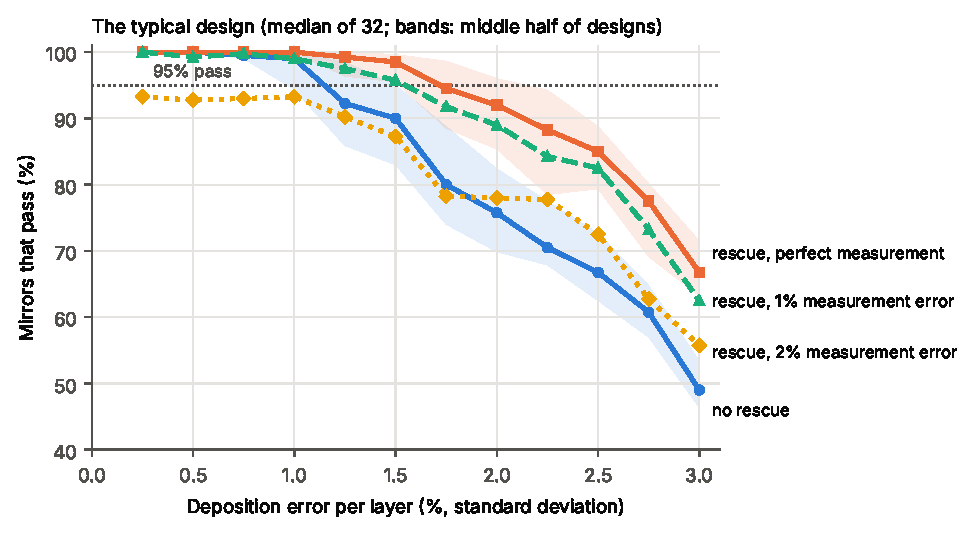
\includegraphics[width=0.75\linewidth]{fig1_typical_design}
\caption{Median pass rate of the 32 designs against deposition error $\sigma$ (independent errors, 200 mirrors per point, top four layers rescued, every mirror rescued). Bands: middle half of the designs, without rescue and with rescue at perfect measurement.}
\label{fig:typical}
\end{figure}

\subsection{How much the rescue raises the tolerable error}
\label{sec:q1}

For each design we found the tolerable error, the deposition error at which the pass rate falls to 95\%, with and without rescue (Fig.~\ref{fig:every}, left).

Without rescue, the median tolerable error was 1.14\%, with the middle half of the designs between 0.96\% and 1.48\%. With rescue and perfect measurement, the median rose to 1.71\% (middle half 1.52--2.19\%). The rescue raised the tolerable error in 30 of the 32 designs, and in 27 of them the uncertainty ranges did not overlap. A sign test gives $p = 2\times10^{-7}$ for 30 increases and 2 decreases. The median per-design gain was 0.59~pp (95\% interval 0.49--0.67~pp; Wilcoxon $p = 10^{-8}$). Expressed as a ratio, the median gain was a factor of 1.43 (95\% interval 1.36--1.56), and it varied between designs from 0.68 to 2.04.

Two designs did worse after rescue. For S1 the tolerable error fell from 0.96\% to 0.66\%, and the uncertainty ranges did not overlap. For E1 it fell from 0.90\% to 0.86\%, with overlapping ranges.

The result does not depend on the three exploratory designs or on the 95\% threshold. Without E1--E3, the median rose from 1.13\% to 1.72\%, with 28 designs up and 1 down. With a 90\% threshold, it rose from 1.43\% to 2.10\%, with 30 up and 2 down.

Designs that were sturdier without rescue did not clearly gain more from it: the rank correlation was $\rho = 0.30$ ($p = 0.09$; corrected $p = 0.6$).

At a single deposition error of 2\%, the median pass rate rose from 76\% without rescue to 92\% with rescue and perfect measurement. All 32 designs had a higher pass rate after rescue, and the number of designs reaching 95\% went from 1 to 13. A second, independent set of 200 mirrors per design gave the same picture: again all 32 designs improved, with a median gain of 12.5 percentage points against 12.2 for the first set.

E3 was also scanned separately with 400 mirrors per point. With 200 mirrors its tolerable error rose from 1.79\% to 2.54\%, and with 400 mirrors from 1.69\% to 2.65\%; the uncertainty ranges overlap. E3 is the third sturdiest of the 32 designs, but its gain ratio with 200 mirrors (1.42) is close to the median.

\begin{figure}[t]
\centering
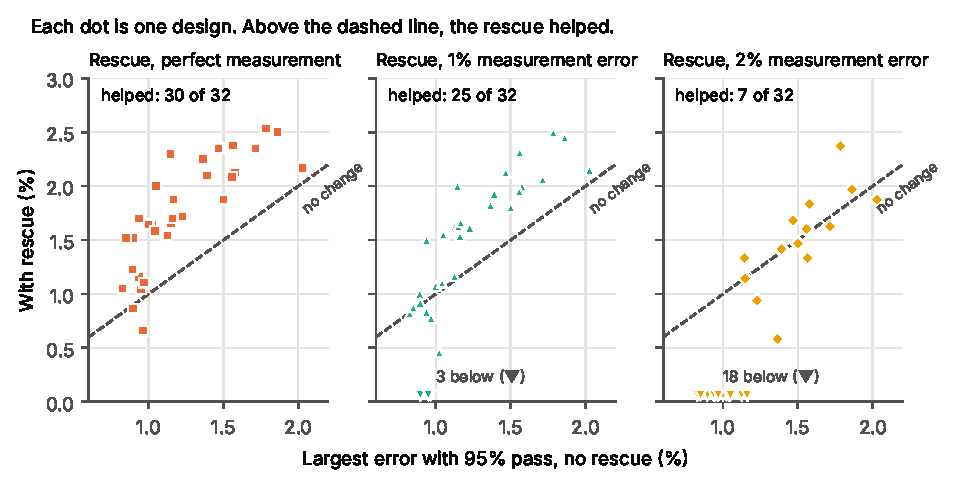
\includegraphics[width=\linewidth]{fig2_every_design}
\caption{Tolerable error of every design with rescue (vertical) against without rescue (horizontal), at three measurement-error levels. Each point is one design; above the dashed line the rescue helped. Triangles at the bottom: designs whose pass rate was below 95\% already at $\sigma = 0.25\%$.}
\label{fig:every}
\end{figure}

\subsection{Effect of measurement error}
\label{sec:measres}

Table~\ref{tab:meas} and Fig.~\ref{fig:every} (middle and right) show how measurement error changes the result. With 1\% measurement error, the rescue still raised the tolerable error in 25 designs and lowered it in 7; the median was 1.58\% (median per-design gain 0.36~pp, 95\% interval 0.07--0.48~pp). With 2\% measurement error, it lowered the tolerable error in 25 designs and raised it in 7. For 18 of the 32 designs, the pass rate with rescue was below 95\% even at the smallest deposition error tested, 0.25\%, so the median tolerable error was below 0.25\%.

At 2\% measurement error the two ways of measuring the effect disagree. The tolerable error is set by small deposition errors, where almost every mirror passes without rescue and the rescue can only do harm. At $\sigma = 2\%$, where there is more to fix, the rescue was roughly neutral: 15 designs had a higher pass rate and 13 a lower one ($p = 0.85$), and mirror by mirror it saved 547 mirrors and broke 609. With a 90\% threshold the tolerable error fell in 19 designs and rose in 13 ($p = 0.4$). With perfect measurement, by contrast, the rescue saved 848 mirrors and broke 38, and was significantly better for 28 designs after correction for multiple tests and significantly worse for none. With 1\% measurement error it saved 759 and broke 190 (25 designs better, 1 worse).

\begin{table}[t]
\centering
\caption{Effect of measurement error on the rescue (independent deposition errors, 32 designs, every mirror rescued). Tolerable error: median and middle half of the designs. ``Clear'': non-overlapping 95\% ranges. Mirrors saved and broken, and designs significantly better or worse after Holm correction, are from the paired comparison at $\sigma = 2\%$. Without rescue, the median tolerable error is 1.14\% (0.96--1.48\%).}
\label{tab:meas}
\footnotesize\setlength{\tabcolsep}{4pt}
\begin{tabular}{lccccc}
\toprule
Measurement & Tolerable error & Raised (clear) / & Sign test & Mirrors saved / & Designs better / \\
error & median (middle half) & lowered (clear) & $p$ & broken & worse \\
\midrule
0\% & 1.71\% (1.52--2.19\%) & 30 (27) / 2 (1) & $2\times10^{-7}$ & 848 / 38 & 28 / 0 \\
1\% & 1.58\% (0.91--1.96\%) & 25 (14) / 7 (3) & 0.002 & 759 / 190 & 25 / 1 \\
2\% & $<0.25\%$ ($<0.25$--1.43\%) & 7 (1) / 25 (18) & 0.002 & 547 / 609 & 1 / 2 \\
\bottomrule
\end{tabular}
\end{table}

To find where the rescue stops helping, we added measurement errors of 0.5\% and 1.5\% (Table~\ref{tab:thresh}). The answer depends on the deposition error. At $\sigma = 1\%$, the rescue helped with measurement errors up to 0.5\%, was neutral at 1\%, and did harm from 1.5\%. At $\sigma = 2\%$, it helped up to 1.5\% and was neutral at 2\%. At $\sigma = 0.25\%$ and 0.5\%, where nearly every mirror passes anyway, any measurement error of 1\% or more did harm. In every case the rescue helped clearly only when the measurement error was smaller than the deposition error. At the points where we repeated the runs with a second set of mirrors, the counts agreed within a few designs (Sec.~\ref{sec:checksres}).

\begin{table}[t]
\centering
\caption{Designs whose pass rate rose / fell with rescue, compared with no rescue on the same 200 mirrors (independent errors, 32 designs, every mirror rescued). Bold: the rescue helped (sign test $p < 0.05$); italic: it did harm.}
\label{tab:thresh}
\footnotesize
\begin{tabular}{lccccc}
\toprule
 & \multicolumn{5}{c}{Measurement error} \\
Deposition error $\sigma$ & 0\% & 0.5\% & 1\% & 1.5\% & 2\% \\
\midrule
0.25\% & 0 / 0 & 0 / 2 & \emph{0 / 13} & \emph{0 / 20} & \emph{0 / 27} \\
0.5\% & 0 / 1 & 0 / 4 & \emph{0 / 18} & \emph{0 / 23} & \emph{0 / 28} \\
1\% & \textbf{18 / 2} & \textbf{16 / 2} & 12 / 8 & \emph{1 / 22} & \emph{0 / 30} \\
2\% & \textbf{32 / 0} & \textbf{31 / 1} & \textbf{28 / 4} & \textbf{22 / 6} & 15 / 13 \\
\bottomrule
\end{tabular}
\end{table}

Part of the harm comes from rescuing every mirror, including mirrors that would have passed. With the gated rule, which rescues only mirrors whose measurements predict a failure, the median tolerable error at 2\% measurement error was 0.93\% instead of below 0.25\%, and 9 designs were ``below'' instead of 18. It was still lower than without rescue (1.14\%): it fell in 21 designs and rose in 10 (Wilcoxon $p = 0.001$). With measurements this poor, the gate itself makes mistakes. It flags good mirrors as failing and rescues them into failure; at $\sigma = 0.25\%$ the median pass rate with the gated rule was 97\%, and one design fell to 72\%. With better measurement, gating gave up part of the gain. Its median tolerable error was 1.59\% with perfect measurement (always rescuing: 1.71\%) and 1.29\% with 1\% measurement error (always rescuing: 1.58\%), because a mirror predicted to pass can still fail once its top layers are deposited with their own errors.

Sturdier designs lost less when measurement got worse. The rank correlation between a design's tolerable error without rescue and its loss in tolerable error from 0\% to 2\% measurement error was $\rho = -0.52$ ($p = 0.002$; corrected $p = 0.02$). This value depends on how ``below'' is entered: with 0.25\% instead of 0 it is $\rho = -0.42$ ($p = 0.02$). At the single deposition error of 2\%, the same correlation, using pass rates, was $\rho = -0.87$ (corrected $p = 10^{-9}$).

\subsection{Quieter and noisier designs}

Without rescue, designs with lower thermal noise tolerated smaller deposition errors: the rank correlation between the noise proxy and the tolerable error was $\rho = 0.67$ ($p = 3\times10^{-5}$; corrected $p = 0.0004$). Much of this correlation comes from the gap between the two noise groups described in Methods. Within the quiet group the correlation was strong ($\rho = 0.72$); within the noisy group it was weak and not significant ($\rho = 0.26$, $p = 0.37$).

Without rescue, the median tolerable errors of the quiet group (18 designs) and the noisy group (14 designs) were 1.00\% and 1.31\%. With rescue and perfect measurement they rose to 1.56\% and 2.09\%, raising the tolerable error in 17 of 18 quiet designs and 13 of 14 noisy ones. The rescued quiet designs therefore tolerated more error than the noisy designs without rescue. With 1\% measurement error, the quiet group fell to 1.05\%, while the noisy group kept 1.86\%. With 2\% measurement error, 14 of the 18 quiet designs were ``below'', against 4 of the 14 noisy designs; the noisy group's median was 1.33\%.

\subsection{Shared deposition errors}

So far each layer had its own error. With a shared error, all 40 layers are off by the same fraction. Table~\ref{tab:shared} and Fig.~\ref{fig:shared} compare the two cases.

At 1\% shared error, the median pass rate without rescue was 66\%. With rescue it rose to 76\% with perfect measurement, 74\% with 1\% measurement error and 69\% with 2\%. At 2\% shared error, the median was 40.5\% without rescue and 48\%, 46\% and 42\% with rescue. With perfect measurement, the rescue raised the pass rate of 31 designs at 1\% shared error and of 29 at 2\%. No design reached a 95\% pass rate: the best after rescue was 91.5\% at 1\% and 56\% at 2\%.

The gain at 1\% shared error is small but consistent. The sign test gives $p = 2\times10^{-8}$. Mirror by mirror, the rescue saved 700 mirrors and broke 29; it was significantly better for 27 designs after correction and significantly worse for none. At 2\% shared error, sturdier designs gained less from the rescue with perfect measurement ($\rho = -0.66$, corrected $p = 0.0005$).

Re-designing more layers helped, but not enough. At 1\% shared error with perfect measurement, the median pass rate was 72.5\% with $k = 2$, 75.5\% with $k = 4$, 79\% with $k = 6$, 83\% with $k = 8$ and 88\% with $k = 12$. Twelve layers did better than four for 31 of the 32 designs, but only 2 designs reached 95\%. A global optimizer did not change this either (Sec.~\ref{sec:checksres}). A shared error scales every layer by the same factor, which shifts the whole spectrum of the coating in wavelength. The top layers can change the phase of the light reflected from the stack beneath them, but they cannot shift that stack's spectrum back, so a few layers can only partly undo the error.

\begin{table}[t]
\centering
\caption{Pass rates under independent and shared deposition errors (32 designs, 200 mirrors each, $k = 4$). Medians over designs; ``raised'' counts designs whose pass rate rose with rescue at perfect measurement.}
\label{tab:shared}
\footnotesize\setlength{\tabcolsep}{4pt}
\begin{tabular}{lccccc}
\toprule
 & No rescue & Rescue, meas.\ 0 / 1 / 2\% & Raised & Best after rescue & Reached 95\% \\
\midrule
Independent, 2\% & 76\% & 92 / 89 / 78\% & 32 & 99.5\% & 13 \\
Shared, 1\% & 66\% & 76 / 74 / 69\% & 31 & 91.5\% & 0 \\
Shared, 2\% & 40.5\% & 48 / 46 / 42\% & 29 & 56\% & 0 \\
\bottomrule
\end{tabular}
\end{table}

\begin{figure}[t]
\centering
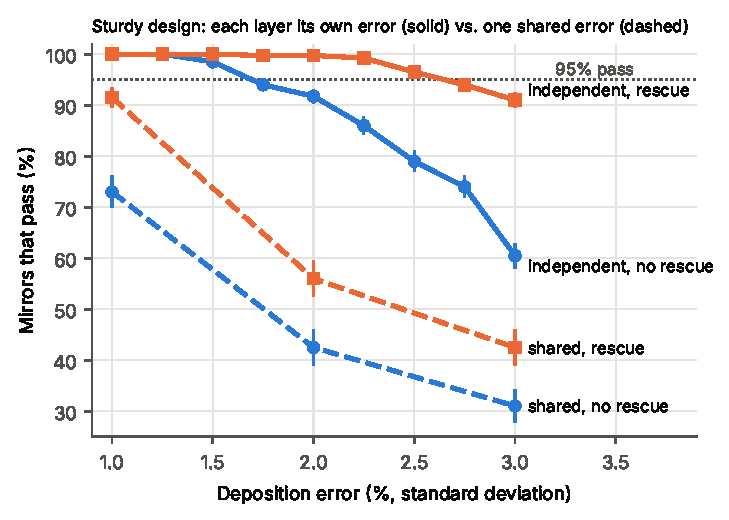
\includegraphics[width=0.9\linewidth]{fig3_shared_error}
\caption{Pass rate of every design without and with rescue ($k = 4$, perfect measurement). Grey lines join the same design; the black line joins the medians. Dotted line: 95\% pass.}
\label{fig:shared}
\end{figure}

\subsection{Number of rescued layers}
\label{sec:kres}

All results above use $k = 4$. Under independent errors of 2\% with perfect measurement, re-designing more layers helped up to about six to eight (Table~\ref{tab:k}). The median pass rate was 92\% with $k = 4$ and 96\% with $k = 8$, and the number of designs reaching 95\% rose from 13 to 20. With $k = 12$ the median fell back to 93.5\%, although the worst design improved. The best $k$ was 6 for 13 designs, 8 for 7 and 12 for 10. The choice $k = 4$ therefore understates what the rescue can do under independent errors.

\begin{table}[t]
\centering
\caption{Pass rate against the number of rescued layers $k$ (32 designs, 200 mirrors each, perfect measurement). Medians over designs.}
\label{tab:k}
\footnotesize
\begin{tabular}{lccccc}
\toprule
$k$ & 2 & 4 & 6 & 8 & 12 \\
\midrule
Independent 2\%: median pass rate & 83\% & 92\% & 95.5\% & 96\% & 93.5\% \\
\quad designs reaching 95\% & 4 & 13 & 20 & 20 & 11 \\
Shared 1\%: median pass rate & 72.5\% & 75.5\% & 79\% & 83\% & 88\% \\
\quad designs reaching 95\% & 0 & 0 & 0 & 0 & 2 \\
\bottomrule
\end{tabular}
\end{table}

\subsection{Why mirrors fail}

We classified the failed mirrors of one design, E3 (Fig.~\ref{fig:failures}). This is a single-design example, not a population result, and it uses its own set of mirrors.

Without rescue, most failures came from 532~nm transmission above its 4\% limit. The rescue removed most of these, and the remaining failures were mainly from 1064~nm transmission above 6~ppm. For example, at 3\% independent error, 40 mirrors failed only the 532~nm limit, 17 only the 1064~nm limit, and 18 both; after rescue these numbers were 5, 16 and 0. At 2\% shared error, the largest group failed both limits at once, and the rescue removed few of these (63 to 55). Failures almost always came from too much transmission, almost never from too little.

\begin{figure}[t]
\centering
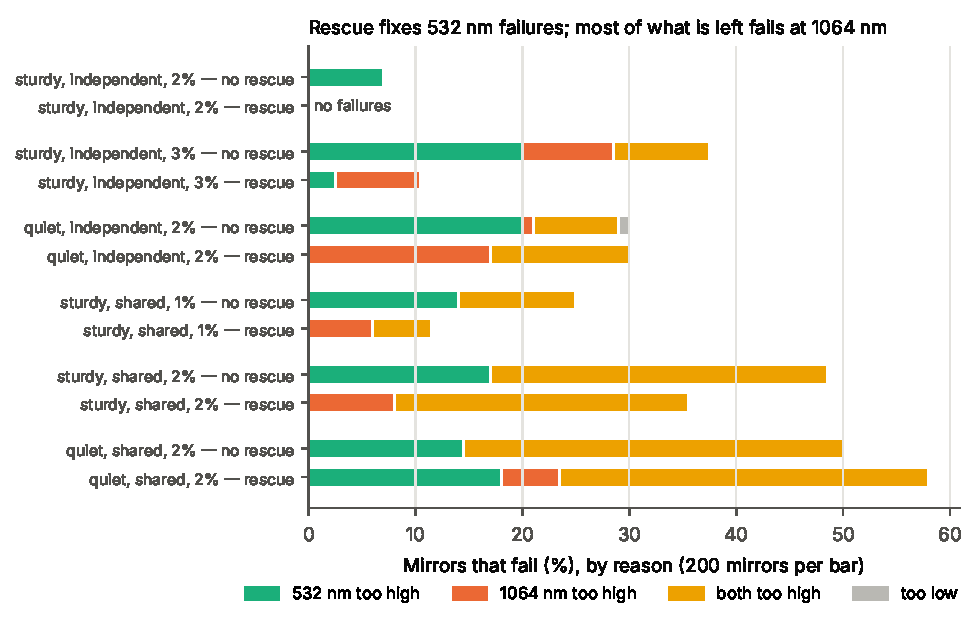
\includegraphics[width=0.75\linewidth]{fig4_failures}
\caption{Failed mirrors of design E3 by the limit they missed, without and with rescue ($k = 4$, perfect measurement), 200 mirrors per bar.}
\label{fig:failures}
\end{figure}

\subsection{Thermal noise}
\label{sec:noiseres}

We computed the full Brownian noise of every mirror at $\sigma = 2\%$ (independent errors), with and without rescue, for all 32 designs. With perfect measurement, the rescue changed the noise at 100~Hz by a median of $-0.02\%$. Ninety percent of mirrors changed by between $-0.63\%$ and $+0.30\%$, and the largest increase for any mirror was 1.09\%. The median of single designs ranged from $-0.24\%$ to $+0.12\%$. With 1\% and 2\% measurement error the medians were $-0.01\%$ and $-0.003\%$, and the largest increases 1.06\% and 1.16\%. Using a substrate Young's modulus of 72.7~GPa instead of 60~GPa changed the median to $-0.01\%$. The noise proxy gave a median of $-0.035\%$ with perfect measurement, twice the full calculation, but both are far below 1\%.

\subsection{Method checks}
\label{sec:checksres}

\emph{Optimizer.} In the first check, on E1 and E3, the slow differential-evolution rescue passed 22 mirrors that L-BFGS-B failed, and L-BFGS-B passed 5 that the slow one failed, out of 1600 (exact McNemar $p = 0.0015$). So the fast optimizer does miss some rescues. Nineteen of the 22 were E1 mirrors under shared errors; for E3 there were 4 disagreements in 800 mirrors. On all 32 designs at 1\% shared error, the two optimizers gave median pass rates of 75.0\% (differential evolution) and 75.5\% (L-BFGS-B). Differential evolution did better for 7 designs, worse for 2, and the same for 23 ($p = 0.18$), and its largest gain on any design was 3.5 percentage points. The fast optimizer's misses are real but too small to explain why shared errors cannot be fixed.

\emph{Second set of mirrors.} We repeated the runs at independent $\sigma = 0.25\%$ and 2\% and shared $\sigma = 1\%$ and 2\%, at all three measurement errors, with a new set of 200 mirrors per design. Every comparison went the same way as with the first set. For example, at independent $\sigma = 2\%$ with 1\% measurement error the rescue raised the pass rate of 29 designs and lowered it for 3 (first set: 28 and 4), and at 2\% measurement error it was neutral again (17 and 14; first set: 15 and 13). The designs that gained most were the same in both sets (rank correlation of the gains between the two sets, 0.64--0.98).

\emph{Size of the Advanced LIGO error.} Scaling all layer thicknesses by a common factor showed how large a systematic error must be to raise the 532~nm transmission tenfold, as happened in the Advanced LIGO end mirrors~\cite{aLIGO2015}: $-2.25\%$ for E3 and $-1.00\%$ for E1. In our model this scaling also pushed the 1064~nm transmission out of its window, which did not happen in the real mirrors. The 1064~nm transmission stayed in range only when one material was scaled; scaling only the silica layers gave 5.21~ppm (E3, $+6.00\%$) and 5.85~ppm (E1, $-1.50\%$). The real coating design differed from ours, so this check shows that errors of a few percent are enough, not that it reproduces the real event.

\section{Discussion}
\label{sec:discussion}

\subsection{The rescue improves tolerance to independent errors}

The main result shows that redesigning the final few layers can make an Advanced LIGO-style mirror more tolerant to independent thickness errors. When we redesigned top 4 layers and made perfect measurements, the median tolerable error increased from 1.14\% to 1.71\%. This is about a 1.4-fold increase. This improvement appeared in 30 of the 32 designs. The 95\% interval for the ratio was 1.36--1.56.

We verified this result with several checks. The result remained unchanged when we removed the three exploratory designs, when we changed the pass threshold from 95\% to 90\%, and when we repeated the simulation with a second set of mirrors. This makes it unlikely that the result came from one unusually good design or one particular set of random errors.

The improvement may be explained by the way independent errors affect the coating. Each layer has its own error, so some layers can become thicker while others become thinner. These changes can partly cancel across the stack. However, the remaining errors can still move the transmission outside the required ranges. By measuring the layers already made and redesigning the final layers, the rescue can correct some of the remaining optical error.

That being said, the improvement was not the same for every design. Two designs became worse (clearly for S1, slightly for E1), and the gain varied widely between designs, from a factor of 0.68 to 2.04. Therefore we cannot guarantee that every coating will become more reliable with this method. However, the improvement across most of the population suggests that the result is not limited to a single design.

The measured gain also depends on how many layers are redesigned. Four layers were chosen after a preliminary test on one design, rather than a full comparison across the population. Later runs showed that redesigning six or eight layers could improve the pass rate further. At 2\% independent deposition error the median pass rate increased from 92\% with four rescued layers to 96\% with eight. This suggests that the four-layer result is not the maximum possible improvement. However, the larger numbers of rescued layers were tested at only a limited number of conditions, so a full comparison is still needed.

\subsection{Measurement accuracy determines whether rescue works}

The most important condition for the rescue method is measurement accuracy. In this method, we used measured layer thicknesses to decide how the remaining layers should change. If the measurements are inaccurate, the optimization may correct errors that are not actually present.

Our results show a clear relationship between deposition error and measurement error. Rescue works best when the measurement error is smaller than the deposition error. For example, at 2\% deposition error, the method still helped when measurement error was up to 1.5\%. But it became roughly neutral when both errors were 2\%. At 1\% deposition error, it helped when measurement error was 0.5\% or less and was neutral at 1\%. It worsened the performance when the measurement error increased further.

This makes sense because the optimization trusts the measurements. When measurement error is small, the measured thicknesses give us a useful picture of the coating that has already been made. The algorithm can then choose final layer thicknesses to compensate for the actual deposition errors. When measurement error becomes large, the algorithm may instead respond to measurement noise. It can change the final layers in the wrong direction and make a passing mirror fail.

Our results also show why a single tolerable-error value does not describe every situation. At 2\% measurement error, the tolerable-error analysis showed a strong decline because it includes small deposition errors, where most mirrors would already pass without rescue. At a fixed 2\% deposition error, however, the rescue was closer to neutral: it saved 547 mirrors and broke 609. These findings are not contradictory. They describe different parts of the error range. Whether the rescue is useful therefore depends partly on the normal accuracy of the coating process.

We further tested whether the damage at 2\% measurement error came mainly from applying rescue to every mirror. A selective method was tested in which rescue was used only when the measured coating was predicted to fail. This reduced the number of designs that performed very poorly at the smallest deposition error. However, it still performed worse than no rescue for more designs than it helped. The reason is that the decision to rescue also depends on imperfect measurements. A mirror may be incorrectly judged as failing or passing. Selective rescue alone cannot solve the problem when the measurements are too inaccurate.

For a real coating process, the important question is therefore whether the monitoring system can measure layer thicknesses more accurately than the deposition process can control them. If it cannot, redesigning the remaining layers may introduce more error than it removes.

\subsection{Quiet designs and manufacturing reliability}

The study also examined whether rescue could make quieter coating designs as reliable as designs with higher thermal noise. This matters because the coating design must balance two goals: low thermal noise and reliable optical performance.

Without rescue, the quieter designs were generally more fragile. Their median tolerable error was 1.00\%, compared with 1.31\% for the noisier group. With perfect measurement, rescue raised the quiet group's median tolerable error to 1.56\%, higher than the noisier group's value without rescue. In principle, this means that a quieter design could become a realistic option without requiring the same level of deposition accuracy.

However, this advantage depended on measurement quality. With 1\% measurement error, the quiet group's median tolerable error fell to 1.05\%. At 2\% measurement error, most quiet designs performed poorly. The quieter designs therefore need more accurate measurements to benefit from rescue.

This means the method does not remove the trade-off between thermal noise and manufacturing reliability. It can reduce that trade-off under good measurement conditions, but it cannot make every quiet design robust. The measurement system may be just as important as the coating design itself.

\subsection{Shared errors require a different correction}

The rescue was much less effective against shared errors. In this model, all layers receive the same relative thickness error. Unlike independent errors, these changes do not partly cancel across the coating. Instead, they shift the whole stack in the same direction.

At 1\% shared error, redesigning four layers improved the median pass rate, but no design reached the required 95\% pass rate. Redesigning more layers improved the result further. With up to 12 layers redesigned, the median pass rate increased from 75.5\% to 88\%, but only two of the 32 designs reached 95\%.

This suggests that the main problem is not simply that four layers are too few. A shared error changes the optical behavior of the whole stack. The final layers can adjust the light reflected from the layers below, but they cannot fully reverse the shift caused by changing the thickness of the entire coating. A global optimizer also gave a similar result, suggesting that the limitation is not only caused by the local optimization method.

This finding is important when considering the Advanced LIGO end-mirror problem. The reported problem involved a systematic thickness error that left the infrared transmission within its required range but increased the green transmission by about an order of magnitude. Our shared-error model suggests that redesigning the final layers could provide some correction, but would not reliably bring the mirrors back to the required pass rate.

However, our model does not reproduce the real Advanced LIGO problem in full. When all layers were scaled in our simulation, the 1064~nm transmission also moved outside its required range. The real coating design was different, and we could not find the size of its thickness error in published work. The comparison therefore supports a similar general point about systematic errors, but it does not establish exactly how the rescue would have performed on the actual Advanced LIGO mirrors.

A more suitable response to shared errors may be to identify and correct the deposition-rate error itself. Measurements from the layers already made could help estimate whether the machine is consistently depositing layers too thick or too thin. The deposition process could then be recalibrated before continuing. This approach was not tested in the present study.

\subsection{Thermal-noise cost}

The rescue did not produce a meaningful increase in thermal noise. Across all 32 designs at 2\% deposition error, the median change was $-$0.02\%. The full thermal-noise calculation also showed that the largest increase for an individual mirror was about 1\%.

This is expected to some extent because the rescue changes only a few layers in a 40-layer coating, so its effect on the total coating noise is limited. More importantly, the optimization does not appear to gain manufacturing tolerance by simply adding more of the higher-loss material.

This result is encouraging because any practical rescue method must preserve the low thermal noise required for gravitational-wave detection. However, the small change in noise should not be interpreted as meaning that thermal noise is irrelevant to the optimization. The result applies to the materials, coating structure, and noise model used here. Other coating designs may behave differently.

\subsection{Practical meaning and future work}

Taken together, our results suggest that the rescue method could be useful for reducing the effect of random layer-to-layer thickness errors. It requires an additional calculation after measuring the deposited layers, but does not require a new coating machine. It may also allow some designs with lower thermal noise to be used without requiring extremely tight deposition control.

However, the method is not a general solution to coating errors. It depends on accurate measurements, and works best against independent errors. It provides only limited correction for shared errors. The results also show that the number of layers redesigned matters. However, we have not established the best number across the full range of conditions yet.

Several steps are needed before the method can be considered for an actual coating process. First, the measurement accuracy and the pattern of measurement errors in real coating machines must be studied. Particularly, measurement errors may be correlated between layers or may build up during a coating run. Second, the method should be tested with mixed error models that include both independent and shared errors. Third, future simulations should include refractive-index errors, material dispersion, absorption, and uneven layer thickness across the mirror.

The rescue strategy itself could also be improved. Redesigning six or eight layers appears promising, but it was tested at only one deposition error for each error model and needs to be tested across all error sizes and measurement conditions. A method that estimates shared errors and adjusts the deposition process may be more useful for systematic errors than simply redesigning the final layers. Finally, experimental work is needed to check whether the redesigned thicknesses can be deposited reliably within the limits of a real coating machine.

Overall, this study shows that redesigning the final layers can improve tolerance to independent thickness errors without a meaningful thermal-noise penalty. The improvement is not automatic: it depends on measurements being more accurate than the deposition process. Shared errors remain a separate problem that requires a different approach.

\section{Limitations}
\label{sec:limitations}

This study has several limitations. Firstly, all results come from computer simulations. We did not make or measure any physical coatings. Therefore, the results show what the rescue method can achieve under our model. But we did not show how it would perform in an actual coating process.

Further, our model includes only thickness errors. Real coatings may have other problems, such as errors in refractive index, material absorption, and variations in layer thickness across the mirror surface. We did not include these effects. We also used the same refractive index for each material at 532~nm and 1064~nm. Real silica and tantala have slightly different refractive indices at these wavelengths. This could change both the original designs and the results of the rescue.

We also simplified the pass test by checking only the transmission at 1064~nm and 532~nm. The real coating specification also considers the electric field at the coating surface and how uniform the coating is across the mirror. We did not consider these requirements in our model.

Our assumptions about measurement errors may also differ from a real coating machine. We tested measurement errors from 0\% to 2\%, but these values were not measured from an actual monitoring system. We assumed that measurement errors were independent from layer to layer. In practice, they may be correlated or build up during a coating run. We also tested two separate deposition-error models: fully independent errors and one shared error across all layers. Real coating processes may contain both types at the same time. In addition, we did not include the fixed part of the deposition error, which can be about 1~nm per layer.

The rescue itself was tested in a limited way. We applied it once before the final few layers were deposited. We did not test applying it after every layer. We also did not test a method that estimates a shared deposition error from the measured layers and corrects the deposition rate.

Most of our results use four redesigned layers. We chose this number based on preliminary tests on one design, rather than a comparison across all 32 designs. Later tests showed that redesigning six or eight layers could improve the pass rate further. However, these tests covered only two error conditions: 2\% independent error and 1\% shared error. We therefore cannot yet say how many layers should be redesigned under different conditions. Similarly, our selective rescue method used the same imperfect measurements to decide whether a mirror needed rescue. A better decision rule that accounts for measurement uncertainty might perform better.

We also did not test whether all redesigned layers would be practical to make. We limited their thicknesses to between 0.5 and 1.5 times their planned values, and the redesigned layers received deposition errors just like the other layers. However, we did not examine how often the optimizer reached these limits or how difficult the new thicknesses would be to deposit in practice.

The results are based on one type of mirror, with two coating materials. We also tested 32 designs generated using the same optimization method and cost function. Three designs came from an earlier run whose original script was not saved. Removing these three designs did not change the main result, but designs generated using a different method may behave differently. We also did not compare the rescue method with designs that were made more robust against thickness errors from the beginning.

Each simulation point used 200 mirrors. This gives some uncertainty in the pass rates, and the uncertainty in an individual tolerable-error value is about 0.1--0.3 percentage points. The medians across all 32 designs are more stable, and a second set of simulated mirrors gave similar results. Still, more simulations would give more precise estimates.

Finally, our fast optimization method does not always find the best possible rescue. In a comparison with a slower, global optimizer, the slower method rescued some mirrors that the fast method missed. However, when we repeated this comparison on all 32 designs at 1\% shared error, the pass rates changed by no more than 3.5 percentage points. The noise proxy used during optimization is also based on physical layer thickness rather than optical thickness, as used in the LIGO specification. Its weight depends on the material values in the software library. We used the full thermal-noise calculation for the reported noise results, but the choice of optimization weights may still affect which designs and rescued coatings are selected.

These limitations mean that the results are evidence that the rescue method can work under certain simulated conditions, not proof that it is ready for use in a real coating process. Further simulations with more realistic error models, followed by experimental tests, are needed to establish its practical value.

\section{Conclusion}
\label{sec:conclusion}

Our study demonstrates that redesigning the final layers of an Advanced LIGO-style mirror coating can improve its tolerance to random thickness errors. When we redesigned the top four layers using perfect measurements, the median tolerable error across 32 designs increased from 1.14\% to 1.71\%, about a 1.4-fold improvement. The rescue improved 30 of the 32 designs. The change in thermal noise was negligible. Tests with six and eight redesigned layers showed that there is room for further improvement.

However, the method depends strongly on measurement accuracy. It worked best when the deposited layers were measured more accurately than they were made. When measurement error became as large as the deposition error, the rescue no longer helped, and when it was larger, the rescue did harm. Using it only on mirrors predicted to fail could not solve this problem completely.

The method was also much less effective against shared errors, where all layers become too thick or too thin by a similar amount. At 1\% shared error, even after redesigning up to 12 layers, only two of the 32 designs reached a 95\% pass rate. Such errors may require correcting the deposition process itself rather than redesigning only the final layers.

Overall, the rescue offers a way to reduce the effect of random layer-to-layer thickness errors while keeping thermal noise nearly unchanged. Its practical value will depend on the accuracy of the coating measurements and the ability to identify the type of error affecting the coating. Further simulations and experimental tests are needed before the method can be applied to real mirror coatings.

% \input{sections/acknowledgments}

% Source: results/stats/stats_checks.txt (below = 0) and results/revision/reanalysis.txt (below = 0.25%).
\appendix
\section{All rank correlations}
\label{app:corr}

Table~\ref{tab:corr} lists all sixteen Spearman correlations we tested. ``Sturdiness'' is a design's tolerable error without rescue (fine scan) or its pass rate without rescue (single points). ``Gain'' is the change from rescue, and ``loss'' is the drop from perfect to 2\% measurement error. Holm correction is over all sixteen. In the fine scan, ``below'' is entered as 0; entering it as 0.25\% gives $\rho = +0.30$, $+0.47$ and $-0.42$ for the last three fine-scan rows (uncorrected $p = 0.09$, 0.006 and 0.02).

\begin{table}[h]
\centering
\caption{Spearman correlations across the 32 designs.}
\label{tab:corr}
\footnotesize
\begin{tabular}{llccc}
\toprule
Run & Correlation & $\rho$ & $p$ & Holm $p$ \\
\midrule
Fine scan & noise proxy vs sturdiness & $+0.67$ & $3\times10^{-5}$ & 0.0004 \\
 & sturdiness vs gain, perfect measurement & $+0.30$ & 0.09 & 0.6 \\
 & sturdiness vs gain, 2\% measurement & $+0.54$ & 0.001 & 0.01 \\
 & sturdiness vs loss & $-0.52$ & 0.002 & 0.02 \\
Independent 2\% & noise proxy vs sturdiness & $+0.66$ & $4\times10^{-5}$ & 0.0005 \\
 & sturdiness vs gain, perfect measurement & $-0.16$ & 0.4 & 0.8 \\
 & sturdiness vs gain, 2\% measurement & $+0.56$ & 0.0008 & 0.008 \\
 & sturdiness vs loss & $-0.87$ & $7\times10^{-11}$ & $10^{-9}$ \\
Shared 1\% & noise proxy vs sturdiness & $+0.50$ & 0.003 & 0.02 \\
 & sturdiness vs gain, perfect measurement & $-0.11$ & 0.5 & 0.8 \\
 & sturdiness vs gain, 2\% measurement & $+0.29$ & 0.1 & 0.6 \\
 & sturdiness vs loss & $-0.88$ & $5\times10^{-11}$ & $9\times10^{-10}$ \\
Shared 2\% & noise proxy vs sturdiness & $-0.23$ & 0.2 & 0.6 \\
 & sturdiness vs gain, perfect measurement & $-0.66$ & $4\times10^{-5}$ & 0.0005 \\
 & sturdiness vs gain, 2\% measurement & $-0.57$ & 0.0007 & 0.007 \\
 & sturdiness vs loss & $-0.29$ & 0.1 & 0.6 \\
\bottomrule
\end{tabular}
\end{table}


\bibliographystyle{unsrtnat}
\bibliography{references}

\end{document}
